\chapter{Introduction/Motivation}
\section{Example usage of different commands}


 \begin{description}
	\item[Abbreviations] \textbackslash acrshort\{DV\} -->  \acrshort{DV}
	\item[Glossary Entry] \textbackslash gls\{Vader\} -->  \gls{Vader}
	\item[To be done note] \textbackslash tbd --> \tbd
	\item[TBD with description] \textbackslash tdb[some Description] --> \tbd[some Description]
	\item[Footnote] \textbackslash footnote\{Not guaranteed that Death Star will be safe\}--> \footnote{Not guaranteed that Death Star will be safe}
	\item[Cites] \textbackslash cite\{deathstar\} --> \cite{deathstar}
 \end{description}
 
 
\section{PGFPlots}

All examples are from PGFPlots \cite{pgfplots:sourceforge}:

Plot \textbf{$f(x) = x^2 - x +4$}:

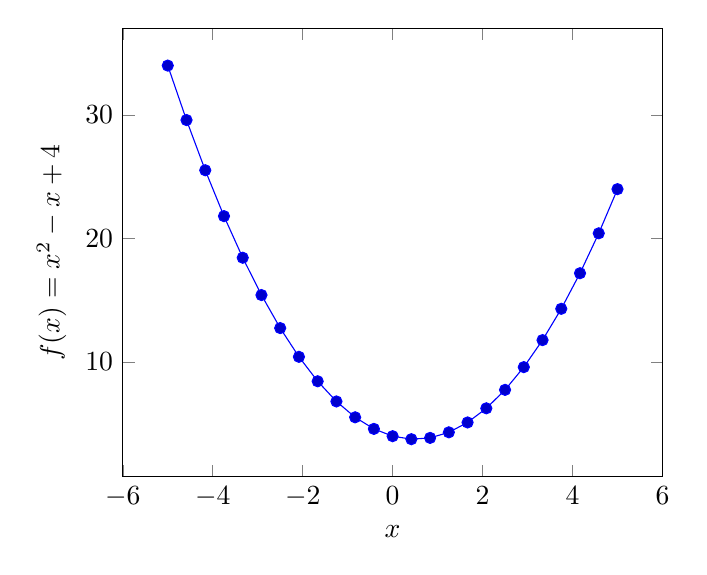
\begin{tikzpicture} 
	\begin{axis}[ xlabel=$x$, ylabel={$f(x) = x^2 - x +4$} ] 
	% use TeX as calculator: 
	\addplot {x^2 - x +4}; 
	\end{axis} 
\end{tikzpicture}


Data from \textbf{diagrams/test-data.csv}:

\pgfplotstableread[col sep=comma]{diagrams/test-data.csv}\loadedtable
\begin{tikzpicture} 
	\begin{axis}[ xlabel=Cost, ylabel=Error] 		
		\addplot[color=red,mark=x] table [x=X,y=Y]{\loadedtable};
	 \end{axis}
\end{tikzpicture}

Data from \textbf{diagrams/test-data2.csv}:

\pgfplotstableread[col sep=&]{diagrams/test-data2.csv}\loadTestData
\begin{tikzpicture}
	\begin{axis}[
	scatter/classes={
		a={mark=square*,blue},
		b={mark=triangle*,red},
		c={mark=o,draw=black}}]
	\addplot[scatter,only marks, scatter src=explicit symbolic] 	table[x=x, y=y, meta=label] {\loadTestData};
	\end{axis}
\end{tikzpicture}


